\documentclass[class=book, crop=false, oneside]{standalone}
\usepackage[subpreambles=true]{standalone}

\usepackage{import}

\graphicspath{{./assets/diagrams/}}

\begin{document}

\chapter*{Translating ER into RM}
The best way to learn this mechanism is to poceed by examples.\\
Let's start with this classic:

\begin{figure}[H]
	\centering
	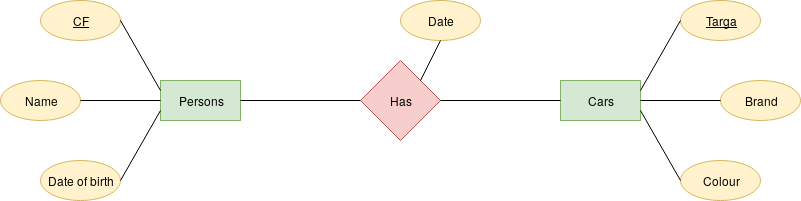
\includegraphics[width=.9\textwidth,keepaspectratio]{diagram1.png}
	\caption{}
	\label{diagram1}
\end{figure}

When we want to translate an Entity Relation Diagram (ERD) into an Relation Model (RM) we have to follow certain rules, let's check them out.
\paragraph*{Rule \#1} every entity becomes a table and its attributes are the table's columns.
\paragraph*{Rule \#2} each relation becomes a table and its attributes are part of the table's columns; also the keys of the entities involved in the relation become columns and they are flagged as Foreign Keys(FK). The FKs must be the table Key.\\
Let's put this in practice:
\vskip 20pt

\begin{minipage}{0.45\textwidth}
	Persons
	\begin{table}[H]
		\centering
		\subimport{assets/tables/}{phc-pers.tex}
	\end{table}
	\texttt{Persons(\underline{CF}, Name, Birth date)}
\end{minipage}
\hspace{.1\textwidth}
\begin{minipage}{.45\textwidth}
	Cars
	\begin{table}[H]
		\centering
		\subimport{assets/tables/}{phc-cars}
	\end{table}
	\texttt{Cars(\underline{Targa}, Brand, Color)}
\end{minipage}
\vskip 20pt
That was pretty easy, wasn't it?\\
Now it's time to draw the relation table:
\vskip 20pt
\begin{minipage}{.7\textwidth}
\begin{table}[H]
	\centering
	\subimport{assets/tables/}{phc-has}
\end{table}
\end{minipage}


% \begin{minipage}{\textwidth}
% 	\vskip 20pt
%
% 	\begin{minipage}{\textwidth}
%
% 		\begin{table}[H]
% 			\centering
% 			\subimport{assets/tables/}{phc-cars_v2}
% 		\end{table}
%
% 	\end{minipage}



\end{document}
